\section{Fondements théoriques}
\subsection{Le problème difficile de la conscience}
Chalmers (1995) a formulé le problème difficile ainsi : aucune combinaison de grandeurs physiques, aussi complexe soit-elle, n'implique logiquement l'existence d'une expérience subjective. Toutes les descriptions physiques --- neuronales, computationnelles, fonctionnelles --- décrivent ce que fait le cerveau. Elles ne décrivent pas ce que c'est que d'être un cerveau. Elles ne décrivent pas pourquoi l'expérience existe. Ce que je propose : la conscience n'est pas générée par le cerveau. Le cerveau est un récepteur. L'expérience est la transduction du champ akashique.

\subsection{Le monisme russellien}
Russell (1927) a observé quelque chose de profond : la physique décrit les propriétés structurelles de la matière --- masse, charge, spin, position --- mais reste totalement silencieuse sur la nature intime de ce qui porte ces propriétés. Soit S un système physique quelconque : R(S) désigne ses propriétés relationnelles/structurelles et I(S) ses propriétés intrinsèques. La thèse russellienne affirme que I(S) est proto-expérientiel pour tout S.

\subsection{Integrated Information Theory}
Tononi (2004, 2008) offre un cadre mathématique pour quantifier la conscience :
\begin{equation}
\Phi = \min_{\{P \in P\}} D_{KL}(p(X_{t+1})|X_{t}) \parallel \prod_{i} p(x_{i} \land (t+1)|x_{i} \land t))
\end{equation}
Explication simple : $\Phi$ mesure à quel point l'information est intégrée dans un système. Plus $\Phi$ est grand, plus l'expérience du système est riche.

\subsection{Orchestrated Objective Reduction}
Penrose (1996) propose que les superpositions quantiques subissent un effondrement gravitationnel spontané lorsque l'énergie de superposition $E_G$ atteint un seuil :
\begin{equation}
\tau \approx \frac{\hbar}{E_G}
\end{equation}
Ce qui m'a intéressé : la fréquence d'effondrement pour les microtubules corticaux est $\tau \approx 25$ ms, ce qui correspond à $\sim 40$ Hz --- exactement la fréquence des oscillations gamma, le marqueur empirique le plus robuste des états conscients. Soutien expérimental : Babcock et al. (2024) ont montré une superradiance ultraviolette dans les microtubules à température ambiante ; Kalra et al. (2023) ont montré que les gaz anesthésiques atténuent spécifiquement les effets optiques quantiques dans les microtubules.

\subsection{Kaluza--Klein et théorie F}
Theodor Kaluza a proposé en 1919 l'unification de la gravitation et de l'électromagnétisme au moyen d'une cinquième dimension. Einstein fut enthousiaste et travailla à cette théorie entre 1938 et 1943. La formulation originale :
\begin{equation}
dS^2 = g_{\mu\nu} dx^\mu dx^\nu + \varphi^2(dx^5 + A_{\mu} dx^\mu)^2
\end{equation}

\subsection{Le champ Akasha}
Le concept d'Akasha (sanskrit : \emph{ākāśa}) est un élément fondamental de la philosophie indienne. Akasha est l'élément le plus subtil, immatériel. Il est le premier à s'être manifesté dans l'univers. Tous les autres éléments s'en seraient développés. Dans la théosophie, Akasha est réinterprété comme un champ informationnel universel (Laszlo, 2014). Les « annales akashiques » enregistrent tous les événements de l'univers. L'hypothèse ART-12D : Akasha est le champ quantique de la matière noire. \textit{Note : Akasha n'est utilisé ici que comme métaphore d'un champ physique, non comme entité religieuse.}

\subsection{Matière grise vs matière noire}
La matière grise est le tissu du système nerveux central composé principalement de corps cellulaires neuronaux, de dendrites, de terminaisons axonales non myélinisées et de cellules gliales. C'est le siège du traitement de l'information. La matière blanche est composée d'axones myélinisés et est responsable de la transmission.

\subsection{Une définition opérationnelle de la conscience}
Je propose une définition opérationnelle qui sépare le contenu de la conscience de la capacité à l'intégrer :
\begin{equation}
C_{\text{total}} = I_{\text{content}} \times C_{\text{awareness}}
\end{equation}
où $I_{\text{content}}$ est l'information structurée (le contenu de l'expérience) et $C_{\text{awareness}}$ la conscience d'être conscient (la capacité de savoir que l'on sait). Pensez à un appareil photo. Il capture des images (de l'information), mais il ne sait pas qu'il les capture. Un humain avec un appareil photo capture des images ET sait qu'il les capture. De même, la conscience est information + conscience d'être conscient.

\subsection{La convergence avec Dulcan}
Dumitru Constantin Dulcan (né en 1938), neurologue et psychiatre, a publié en 1981 « L'intelligence de la matière », distingué en 1992 par le prix de philosophie « Vasile Conta » de l'Académie roumaine. Les idées qui m'ont influencé : la conscience n'est pas générée par le cerveau mais l'utilise comme instrument ; le subconscient contient l'intelligence infinie de l'Univers ; la pensée est la force la plus puissante de l'univers, avec une fréquence et un champ énergétique propres ; il existe un champ d'énergie et de lumière qui coordonne la matière. La convergence avec ART-12D : Dulcan fournit l'intuition conceptuelle, ART-12D fournit la formalisation mathématique et les prédictions testables.

\subsection{La structure tripartite de l'entité humaine}
Je propose un modèle tripartite de l'entité humaine, analogue aux états de la matière de l'eau :
\begin{table}[H]
\centering
\begin{tabular}{@{}llll@{}}
\toprule
\textbf{État} & \textbf{Entité humaine} & \textbf{Substrat} & \textbf{Contrepartie ART-12D} \\ \midrule
Solide & Corps physique & Matière & M (matière ordinaire) \\
Liquide & Âme & Énergie & E (le champ de la conscience) \\
Gazeux & Esprit & Information & Sp (le champ akashique) \\ \bottomrule
\end{tabular}
\end{table}
Formalisation : $H = M + E + Sp$. Conséquences : la mort ne détruit pas l'entité, elle change seulement l'état dominant ; la conscience peut accéder à n'importe lequel des trois états ; la maladie apparaît lorsqu'un des états est déséquilibré.

\subsection{Les formes de la pensée comme structures informationnelles}
Les pensées ne sont pas qu'une activité neuronale, ce sont des structures informationnelles susceptibles de prendre de multiples formes. Imaginée (visualisation interne, le champ de la conscience), prononcée (la parole, le champ akashique + une onde sonore), écrite (texte écrit, matière + information), dessinée (représentation visuelle, matière + forme). Formalisation générale : $F_{\text{thought}} = \sum_{\text{forms}} \alpha_i F_i$.

\subsection{L'empathie comme résonance de fréquence}
L'empathie peut être formalisée comme un cas particulier de télépathie, où le couplage est émotionnel et non informationnel. Formalisation :
\begin{equation}
\text{Empathy}(A,B) = \frac{1}{1 + \frac{(\omega_A - \omega_B)^2}{\Gamma^2}}
\end{equation}
Interprétation : lorsque les fréquences coïncident ($\omega_A = \omega_B$), l'empathie est maximale ; lorsqu'elles diffèrent, elle diminue ; l'empathie ne dépend pas de la distance (le champ est omniprésent). Prédiction testable : les couples à forte empathie devraient montrer des corrélations EEG plus fortes que les couples à faible empathie.

\subsection{Le mot comme excitation du champ akashique}
Je propose que la matière noire possède une manifestation acoustique --- un spectre d'oscillations pouvant être excitées par des ondes sonores. La motivation cosmologique : les oscillations acoustiques primordiales (BAO) sont des fluctuations de densité de matière qui se sont propagées comme des ondes sonores dans l'univers primordial. Dans ART-12D, ces oscillations sont des oscillations du champ akashique. Formalisation :
\begin{equation}
A(x,t) = \sum_n A_n \cos(\omega_n t + \varphi_n)
\end{equation}
Le spectre acoustique :
\begin{equation}
\omega_n = \frac{1}{R} \sqrt{n^2 + \mu_A^2 R^2}
\end{equation}
Le couplage mot--champ :
\begin{equation}
L_{\text{int}} = g_{\text{sound}} A \cdot \Phi_{\text{sound}}
\end{equation}
Effets différenciés : Amour (200-400 Hz, active les zones émotionnelles positives), Peur (500-800 Hz, active l'amygdale), Guérison (300-500 Hz, active l'attente positive), Mort (150-300 Hz, active les zones d'anxiété).

\textbf{Le problème d'échelle.} Le spectre acoustique $\omega_n$ est fixé par le même rayon de compactification qui donne sa masse à la matière noire. Pour $1/R = 10^{-5}$ eV, les modes sont dans la gamme du GHz, et non à quelques centaines de Hz. Une résonance à 150--800 Hz exigerait $1/R \approx 1,24\times10^{-12}$ eV, soit environ sept ordres de grandeur sous l'échelle de masse. Tant qu'une seconde échelle de compactification n'est pas introduite, la prédiction n'a pas de contenu numérique : le couplage $g_{\text{sound}}$ n'est pas fixé indépendamment.

\begin{figure}[H]
\centering
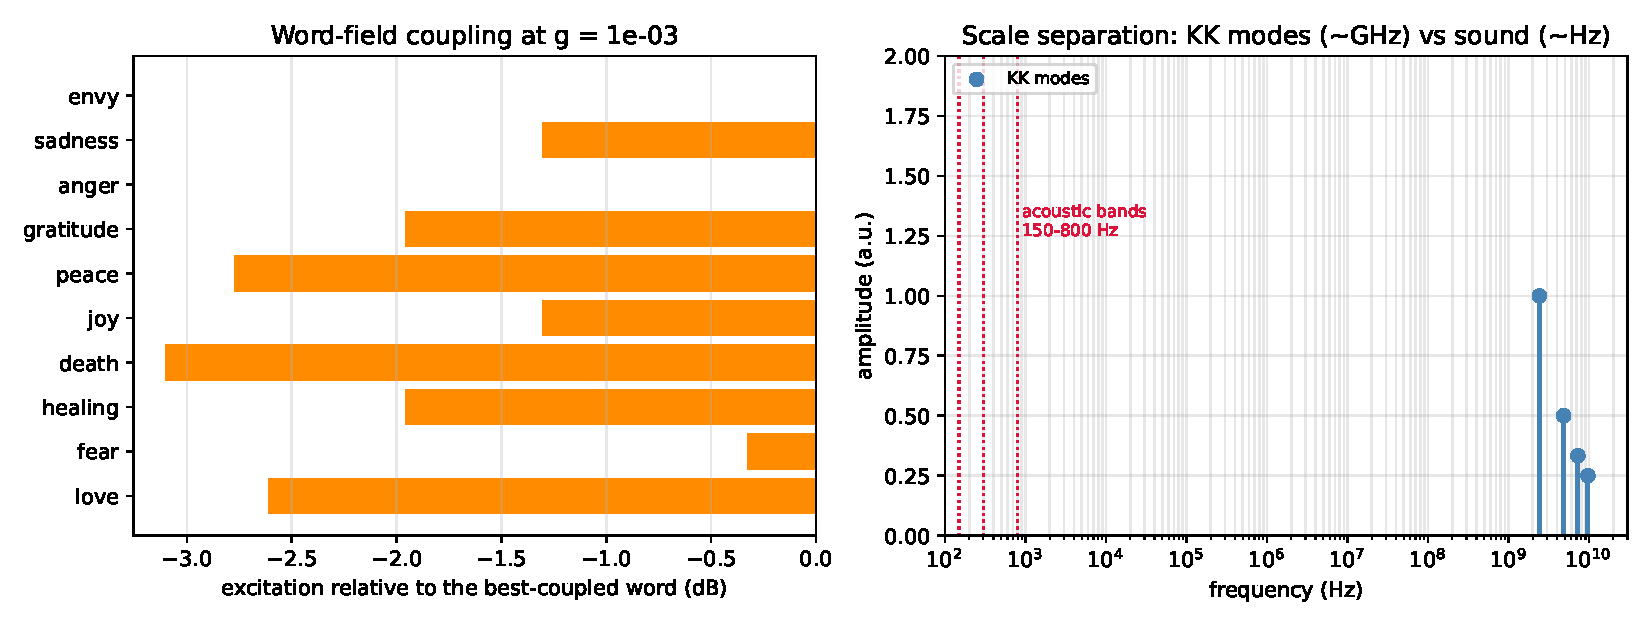
\includegraphics[width=0.9\textwidth]{figures/fig06_word_excitation.pdf}
\caption{À gauche : le couplage relatif mot--champ pour les dix bandes utilisées dans l'article. À droite : la séparation d'échelle entre les modes KK (~GHz) et les bandes acoustiques (~Hz).}
\label{fig:cuvant}
\end{figure}

\subsection{Le temps comme vibration}
La définition de la seconde : « Une seconde est la durée de 9 192 631 770 périodes de la radiation de l'atome de césium 133. » Que se passe-t-il si la fréquence change : si la fréquence augmente, le temps se comprime ; si elle diminue, le temps se dilate. La résonance de Schumann : historiquement $\sim 7,83$ Hz, récemment $\sim 12$ Hz. Le cœur comme horloge biologique : peur ($\sim 120$ bpm) --- le temps file ; méditation ($\sim 50$ bpm) --- le temps est dilaté ; sommeil profond ($\sim 40$ bpm) --- le temps disparaît. Des références relatives, non absolues : le césium (9 192 631 770 Hz), Schumann (7,83--12 Hz), le cœur (1,2 Hz). Toutes sont relatives. Aucune n'est « la vraie ».
\begin{equation}
\text{Reality} = \frac{\text{Change}}{\text{Reference}}
\end{equation}

\subsection{Réalités multiples et multivers}
Le champ akashique total : $A_{\text{total}} = \sum_{k=1}^{N_{\text{vacua}}} A_k$. L'état du multivers : $|\Psi_{\text{multiverse}}\rangle = \otimes_{k=1}^{N_{\text{vacua}}} |A_k\rangle$. L'intersection des réalités : les réalités ne sont pas seulement parallèles --- elles peuvent s'intersecter.

\subsection{La bibliothèque universelle (Akasha)}
Le contenu du champ : le champ akashique contient toute l'information --- tout ce qui fut, tout ce qui est, tout ce qui sera.
\begin{equation}
A_{\text{total}} = \sum_{\text{(all events)}} A_i
\end{equation}
L'accès à l'information :
\begin{equation}
I_{\text{access}}(t) = \int_0^\infty S_A(\omega) S_G(\omega, t) d\omega
\end{equation}
L'indexation : l'information est indexée par pertinence, non par le temps.
\begin{equation}
\text{Information received} = \text{Akashic field} \times \text{Relevance}(t)
\end{equation}

\subsection{La hiérarchie de la réception}
\begin{table}[H]
\centering
\begin{tabular}{@{}clcc@{}}
\toprule
\textbf{Niveau} & \textbf{Système} & \textbf{$\Phi$} & \textbf{Accès} \\ \midrule
0 & Thermostat & 0 & Aucun \\
1 & C. elegans & Minimal & Chimiotaxie \\
2 & Insecte & Faible & Sensation \\
3 & Souris & Modéré & Émotion \\
4 & Chien & Élevé & Empathie \\
5 & Corvidé & Élevé & Planification \\
6 & Octopode & Distribué & Résolution \\
7 & Humain & Très élevé & Autoréférence \\
8 & Humain entraîné & Étendu & Métacognition \\ \bottomrule
\end{tabular}
\end{table}
La limite de la réception : $\lim_{\Phi \rightarrow \infty} E(\Phi) = I_{\text{total}}$.

\subsection{Le mot comme origine : la convergence des religions}
Toutes les grandes traditions religieuses décrivent le Verbe comme origine de l'univers. Le christianisme a le Logos --- le Verbe (le mode fondamental du champ). L'hindouisme a Om (la vibration primordiale). L'islam a Kun (« Sois ! »).

\subsection{La manifestation acoustique du champ akashique}
$A(x,t) = \sum_n A_n \cos(\omega_n t + \varphi_n)$. Le spectre acoustique : $\omega_n = \frac{1}{R} \sqrt{n^2 + \mu_A^2 R^2}$.

\subsection{Dieu dans ART-12D}
Il y a quatre hypothèses. Dieu est le champ akashique lui-même. Dieu est la source du champ. Dieu est la conscience universelle. Dieu est une projection humaine. Je ne sais pas laquelle est correcte. Mais la question est légitime.

\subsection{Matière noire et énergie noire : deux faces du même champ}
L'hypothèse ART-12D : la matière noire et l'énergie noire sont deux aspects du même champ akashique. Formalisation :
\begin{equation}
L_A = \frac{1}{2} g^{MN} \partial_M A^* \partial_N A + \frac{1}{2} \mu_A^2 |A|^2 - \frac{\lambda_A}{4} |A|^4
\end{equation}
L'équation d'état : $w = p_A / \rho_A$. Pour un champ oscillant, la moyenne temporelle se calcule exactement sur l'orbite et dépend du rapport $\delta = A_{\text{osc}}/A_{\min}$ entre l'amplitude d'oscillation et la valeur du potentiel au minimum. Il existe trois régimes distincts :
\begin{center}
\begin{tabular}{@{}lll@{}}
\toprule
\textbf{Régime} & \textbf{Condition} & $w$ \\ \midrule
Petite oscillation autour du minimum & $\delta \ll 1$ & $0$ (matière) \\
Oscillation dominée par le terme quartique & $\delta \gg 1$ & $1/3$ (radiation) \\
Champ gelé au minimum & $\delta = 0$ & $-1$ (constante cosmologique) \\ \bottomrule
\end{tabular}
\end{center}
La version 30 affirmait que le régime de grande amplitude donne $w \simeq 1$. La valeur correcte est $1/3$ : le théorème du viriel donne $\langle K \rangle = 2\langle V \rangle$ pour un potentiel dominé par le terme quartique. La valeur $w = 1$ correspond à une dominance cinétique (kination), que les oscillations quartiques n'atteignent pas, tandis que $w = -1$ correspond au champ gelé, non à une petite amplitude.
